\documentclass{standalone}
\usepackage{pgfplots}
\pgfplotsset{compat=1.17}

\begin{document}

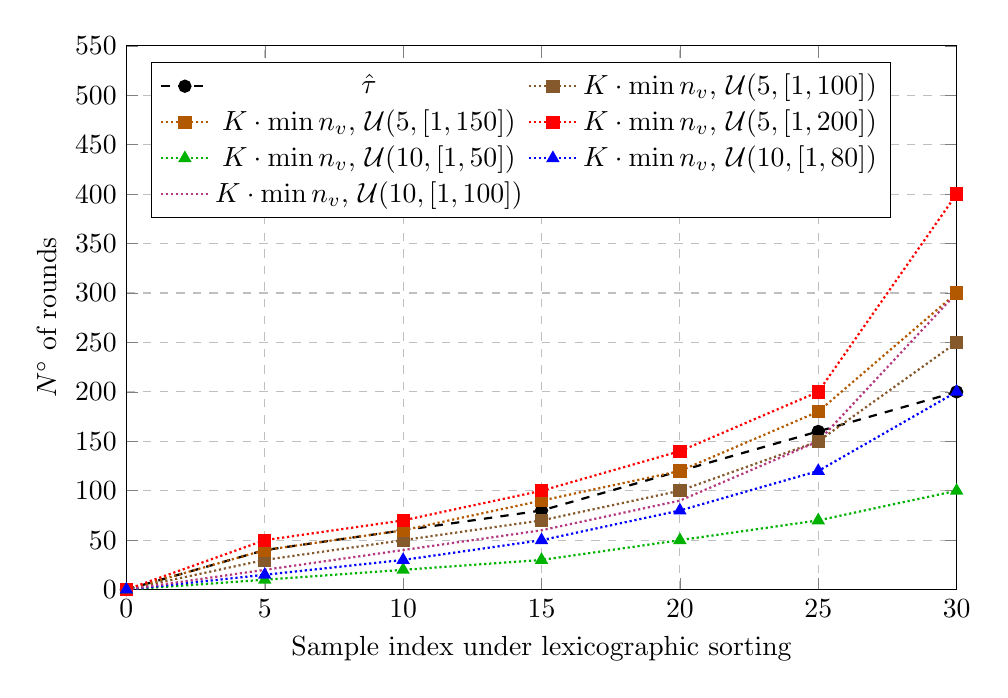
\begin{tikzpicture}
    \begin{axis}[
        width=\textwidth,
        height=0.7\textwidth,
        xlabel={Sample index under lexicographic sorting},
        ylabel={$N^\circ$ of rounds},
        xmin=0, xmax=30,
        ymin=0, ymax=550,
        xtick distance=5,
        ytick distance=50,
        legend pos=north west,
        legend columns=2,
        grid=major,
        grid style=dashed,
        every axis plot post/.append style={
            mark options={solid},
            thick,
        },
    ]

    % Plot for \hat{\tau} and K \cdot \min n_v for different U distributions
    \addplot+[mark=*, black, dashed] coordinates {
        (0, 0) (5, 40) (10, 60) (15, 80) (20, 120) (25, 160) (30, 200)
    };
    \addlegendentry{$\hat{\tau}$};

    \addplot+[mark=square*, brown!70!black, densely dotted] coordinates {
        (0, 0) (5, 30) (10, 50) (15, 70) (20, 100) (25, 150) (30, 250)
    };
    \addlegendentry{$K \cdot \min n_v$, $\mathcal{U}(5,[1,100])$};

    \addplot+[mark=square*, orange!70!black, densely dotted] coordinates {
        (0, 0) (5, 40) (10, 60) (15, 90) (20, 120) (25, 180) (30, 300)
    };
    \addlegendentry{$K \cdot \min n_v$, $\mathcal{U}(5,[1,150])$};

    \addplot+[mark=square*, red, densely dotted] coordinates {
        (0, 0) (5, 50) (10, 70) (15, 100) (20, 140) (25, 200) (30, 400)
    };
    \addlegendentry{$K \cdot \min n_v$, $\mathcal{U}(5,[1,200])$};

    \addplot+[mark=triangle*, green!70!black, densely dotted] coordinates {
        (0, 0) (5, 10) (10, 20) (15, 30) (20, 50) (25, 70) (30, 100)
    };
    \addlegendentry{$K \cdot \min n_v$, $\mathcal{U}(10,[1,50])$};

    \addplot+[mark=triangle*, blue, densely dotted] coordinates {
        (0, 0) (5, 15) (10, 30) (15, 50) (20, 80) (25, 120) (30, 200)
    };
    \addlegendentry{$K \cdot \min n_v$, $\mathcal{U}(10,[1,80])$};

    \addplot+[mark=star*, magenta!70!black, densely dotted] coordinates {
        (0, 0) (5, 20) (10, 40) (15, 60) (20, 90) (25, 150) (30, 300)
    };
    \addlegendentry{$K \cdot \min n_v$, $\mathcal{U}(10,[1,100])$};

    \end{axis}
\end{tikzpicture}

\end{document}